

% ***********************************************************
% ******************* PHYSICS HEADER ************************
% ***********************************************************
% Version 2
\documentclass[12pt]{article} 
\usepackage{amsmath} % AMS Math Package
\usepackage{amsthm} % Theorem Formatting
\usepackage{amssymb}	% Math symbols such as \mathbb
\usepackage{graphicx} % Allows for eps images
\usepackage{multicol} % Allows for multiple columns
\usepackage[dvips,letterpaper,margin=0.75in,bottom=0.5in]{geometry}
 % Sets margins and page size
\pagestyle{empty} % Removes page numbers
\makeatletter % Need for anything that contains an @ command 
\renewcommand{\maketitle} % Redefine maketitle to conserve space
{ \begingroup \vskip 10pt \begin{center} \large {\bf \@title}
	\vskip 10pt \large \@author \hskip 20pt \@date \end{center}
  \vskip 10pt \endgroup \setcounter{footnote}{0} }
\makeatother % End of region containing @ commands
\renewcommand{\labelenumi}{(\alph{enumi})} % Use letters for enumerate
% \DeclareMathOperator{\Sample}{Sample}
\let\vaccent=\v % rename builtin command \v{} to \vaccent{}
\renewcommand{\v}[1]{\ensuremath{\mathbf{#1}}} % for vectors
\newcommand{\gv}[1]{\ensuremath{\mbox{\boldmath$ #1 $}}} 
% for vectors of Greek letters
\newcommand{\uv}[1]{\ensuremath{\mathbf{\hat{#1}}}} % for unit vector
\newcommand{\abs}[1]{\left| #1 \right|} % for absolute value
\newcommand{\avg}[1]{\left< #1 \right>} % for average
\let\underdot=\d % rename builtin command \d{} to \underdot{}
\renewcommand{\d}[2]{\frac{d #1}{d #2}} % for derivatives
\newcommand{\dd}[2]{\frac{d^2 #1}{d #2^2}} % for double derivatives
\newcommand{\pd}[2]{\frac{\partial #1}{\partial #2}} 
% for partial derivatives
\newcommand{\pdd}[2]{\frac{\partial^2 #1}{\partial #2^2}} 
% for double partial derivatives
\newcommand{\pdc}[3]{\left( \frac{\partial #1}{\partial #2}
 \right)_{#3}} % for thermodynamic partial derivatives
\newcommand{\ket}[1]{\left| #1 \right>} % for Dirac bras
\newcommand{\bra}[1]{\left< #1 \right|} % for Dirac kets
\newcommand{\braket}[2]{\left< #1 \vphantom{#2} \right|
 \left. #2 \vphantom{#1} \right>} % for Dirac brackets
\newcommand{\matrixel}[3]{\left< #1 \vphantom{#2#3} \right|
 #2 \left| #3 \vphantom{#1#2} \right>} % for Dirac matrix elements
\newcommand{\grad}[1]{\gv{\nabla} #1} % for gradient
\let\divsymb=\div % rename builtin command \div to \divsymb
\renewcommand{\div}[1]{\gv{\nabla} \cdot #1} % for divergence
\newcommand{\curl}[1]{\gv{\nabla} \times #1} % for curl
\let\baraccent=\= % rename builtin command \= to \baraccent
\renewcommand{\=}[1]{\stackrel{#1}{=}} % for putting numbers above =
\newtheorem{prop}{Proposition}
\newtheorem{thm}{Theorem}[section]
\newtheorem{lem}[thm]{Lemma}
\theoremstyle{definition}
\newtheorem{dfn}{Definition}
\theoremstyle{remark}
\newtheorem*{rmk}{Remark}

% ***********************************************************
% ********************** END HEADER *************************
% ***********************************************************
\usepackage{graphicx}
\begin{document}

\title{Solution To Take-Home Problem Number 4}
\author{Anurag Pallaprolu\\2012B5A3405P\\SK 207, BITS Pilani}
\maketitle


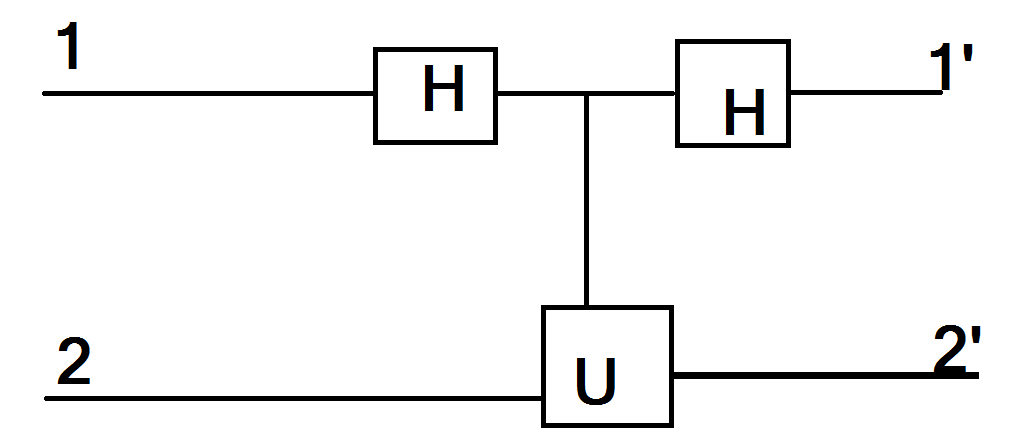
\includegraphics[scale=0.5]{imgsrc.png}
\section{The Question}
This document essentially deals with solving the problem, whose figure is given above. Two qubits $\ket{0}$ and a random qubit $\ket{x}$ are given to us which go through paths 1 and 2 respectively. Then, there are two Hadamard gates and one unknown unitary gate $\v{U}$ is given. It is also said that if $\v{U}$ is seen as an observable then, it has eigenvalues +1 and -1.  The two qubit system is sent through the gated circuit and then the output at 1' is then measured as an eigenstate of $\sigma_{z}$. Now, the question at hand, to be proven is that, when the measuring device measures either a +1 or a -1 eigenvalue of  $\sigma_{z}$, then the output state of $\ket{x}$ at 2' will be an eigenstate of $\v{U}$ corresponding to the eigenvalue +1 or -1.
\section{The Solution}
Now the entire two qubit system is seen as a tensor product of the individual qubits i.e., $\ket{0} \otimes \ket{x}$. If $\ket{x}$ is assumed to be in the standard eigenbasis i.e, $\ket{0}$ and $\ket{1}$, then it can always be written as $$\ket{x} = \alpha\ket{0} + \beta\ket{1}$$. Now, with this in hand, we immediately take the Kronecker product of the two qubits, which follows by definition: $$\ket{0} \otimes \ket{x} = \alpha\ket{00} + \beta\ket{01}$$. Let us for simplicity name this mixed state as $\ket{\Psi}$. The sequentially next logical operation is the action of the first Hadamard gate on the product state. Specifically, it is supposed to act only on the first qubit part of the pair. Taking $H\ket{\Psi}$ we can see that, by definition of the Hadamard gate, this simplifies to $$H\ket{\Psi} = H\alpha\ket{00} +H \beta\ket{01}$$. Then, operating on the first qubit,: $$\alpha(\sqrt{\frac{1}{2}}\ket{0}+\ket{1}) \otimes \ket{0} + \beta(\sqrt{\frac{1}{2}}\ket{0}-\ket{1}) \otimes \ket{1}$$
 A simplification is visible, which immediately confirms the following expression $$H\ket{\Psi} = \sqrt{\frac{1}{2}}(\alpha\ket{00}+\alpha\ket{10} + \beta\ket{01} - \beta\ket{11})$$. Now the pair passes through the $\v{U}$ gate. This is a new and an undefined gate, but it is given to be unitary and hermitian. Hence, we can assume that, it works like any standard logic gate and can be operated linearly on our product pair. Let us not think about the eigenvalues, eigenvectors or eigenbasis of $\v{U}$ for now and just look at it as any hermitian operator on $\ket{x}$. So, directly operating it on $\ket{\Psi}$ yields $$ \v{U}\ket{\Psi} = \v{U}( \sqrt{\frac{1}{2}}(\alpha\ket{00}+\alpha\ket{10} + \beta\ket{01} - \beta\ket{11}))$$. It can be seen that, we can split the pair again into tensor product forms.  $$ \v{U}\ket{\Psi} =  \sqrt{\frac{1}{2}}(\alpha\v{U}\ket{00}+\alpha\v{U}\ket{10} + \beta\v{U}\ket{01} - \beta\v{U}\ket{11}))$$
This then simplifies to $$\sqrt{\frac{1}{2}}(\ket{0} \otimes \v{U}(\alpha\ket{0} + \beta\ket{1})) + \sqrt{\frac{1}{2}}(\ket{1} \otimes \v{U}(\alpha\ket{0} - \beta\ket{1}))$$. By now, it must be clear that we have reached a point where, we have again seen the form of a qubit exactly in the form of $\ket{x}$. Replacing the corresponding symbols and also noting the fact that $$\alpha\ket{0} - \beta\ket{1} = \sigma_{z}\ket{x}$$. Finally, we have the following equality:
$$ \v{U}\ket{\Psi} = \sqrt{\frac{1}{2}}(\ket{0} \otimes \v{U}\ket{x}) + \sqrt{\frac{1}{2}}(\ket{1} \otimes \v{U}\sigma_{z}\ket{x})$$
Now another Hadamard gate awaits to act on the first qubit. Symbolically, $$H \v{U}\ket{\Psi} = H(\sqrt{\frac{1}{2}}(\ket{0} \otimes \v{U}\ket{x}) + \sqrt{\frac{1}{2}}(\ket{1} \otimes \v{U}\sigma_{z}\ket{x}))$$
$$H(\sqrt{\frac{1}{2}}(\ket{0} \otimes \v{U}\ket{x}) + \sqrt{\frac{1}{2}}(\ket{1} \otimes \v{U}\sigma_{z}\ket{x})) = \sqrt{\frac{1}{2}}(\sqrt{\frac{1}{2}}\ket{0}+\ket{1} \otimes \v{U}\ket{x}) + \sqrt{\frac{1}{2}}(\sqrt{\frac{1}{2}}\ket{0}-\ket{1} \otimes \v{U}\sigma_{z}\ket{x})$$

This large expression is actually quite simple, if the pattern in it can be observed. Rearranging the terms
$$H \v{U}\ket{\Psi} = \frac{1}{2}(\ket{0} \otimes(\v{U}\ket{x}+\v{U}\sigma_{z}\ket{x}) + \ket{1} \otimes(\v{U}\ket{x}-\v{U}\sigma_{z}\ket{x}))$$.

The crucial point to be noted is that the standard basis i.e $ \ket{0}$ and $\ket{1}$ is also the eigenbasis of $\sigma_{z}$. Let us call the eigenkets of $\sigma_{z}$ as $\ket{+}$ and $\ket{-}$. Then, we can see that $$H \v{U}\ket{\Psi} = \frac{1}{2}(\ket{0} \otimes(\v{U}\ket{x}+\v{U}\sigma_{z}\ket{x}) + \ket{1} \otimes(\v{U}\ket{x}-\v{U}\sigma_{z}\ket{x})) = \frac{1}{2}(\ket{+} \otimes(\v{U}\ket{x}+\v{U}\sigma_{z}\ket{x}) + \ket{-} \otimes(\v{U}\ket{x}-\v{U}\sigma_{z}\ket{x}))$$

The final step is the measurement of the first qubit using $\sigma_{z}$ as the observable. This implies that we have to multiply our final pair $H \v{U}\ket{\Psi}$ with the eigenkets of the observable. Operating with $\bra{+}$  we get $$\bra{+}H\v{U}\ket{\Psi} = \bra{+}(\frac{1}{2}(\ket{+} \otimes(\v{U}\ket{x}+\v{U}\sigma_{z}\ket{x}) + \ket{-} \otimes(\v{U}\ket{x}-\v{U}\sigma_{z}\ket{x}))$$. Noting that $\bra{+}\ket{+} = 1$ and $\bra{+}\ket{-} = 0$ we can simplify the expression to: $$\bra{+}H\v{U}\ket{\Psi} = (\frac{1}{2}( \v{I} \otimes(\v{U}\ket{x}+\v{U}\sigma_{z}\ket{x}) $$. Now, replacing $\ket{x} = \alpha\ket{+} + \beta\ket{-}$ we can see that $$(\frac{1}{2}( \v{I} \otimes(\v{U}\ket{x}+\v{U}\sigma_{z}\ket{x}) = \frac{1}{2}(\v{U}(\alpha\ket{+} + \beta\ket{-})+\v{U}(\alpha\ket{+} - \beta\ket{-}))$$.
$$\bra{+}H\v{U}\ket{\Psi} = \alpha\v{U}\ket{+}$$. This is where we stop. Notice that, we have reached here only after the operation of $\bra{+}$ on our qubit product. Hence, this should represent as to what was left of the second qubit, as the measurement was on the first one. It is clear from the above expression that the second qubit is ultimately $\v{U}\ket{+}$. Assuming that the eigenbasis of $\v{U}$ can always be seen in the standard or the $\sigma_{z}$ eigenbasis, we can conclude that, whenever we measure $\bra{+}$ on the product, we get the corresponding eigenket for $\v{U}$. QED.
\end{document}